\documentclass[UTF8,a4paper,12pt,oneside]{ctexrep}

\usepackage{geometry}
\usepackage{setspace}
\usepackage{booktabs}
\usepackage{longtable}
\usepackage{tabularx}
\usepackage{array}
\usepackage{xurl}
\usepackage{enumitem}
\usepackage{xcolor}
\usepackage{hyperref}
\usepackage{fancyhdr}
\usepackage{titlesec}
\usepackage{float}
\usepackage{graphicx}
\usepackage{listings}

\geometry{left=2.8cm,right=2.8cm,top=2.8cm,bottom=2.8cm}
\onehalfspacing
\setlength{\parindent}{2em}
\setlength{\parskip}{0.25em}
\setlist[itemize]{leftmargin=2.5em}
\setlist[enumerate]{leftmargin=2.7em}

\setCJKmainfont{NotoSerifCJKsc-Regular.otf}[
  Path = ./font/,
  BoldFont = NotoSerifCJKsc-Bold.otf
]

\setmonofont{consola.ttf}[
  Path = ./font/, 
  BoldFont = consolab.ttf,
  ItalicFont = consolai.ttf,
  BoldItalicFont = consolaz.ttf
]

\hypersetup{
  colorlinks=true,
  linkcolor=black,
  urlcolor=blue,
  citecolor=black,
  pdfauthor={seccomp-privacy-platform team},
  pdftitle={面向电商隐私分析场景的 SSE + PJC 平台设计与实现}
}

\pagestyle{fancy}
\setlength{\headheight}{15pt}
\fancyhf{}
\fancyhead[C]{面向电商隐私分析场景的 SSE + PJC 平台设计与实现}
\fancyfoot[C]{\thepage}
\renewcommand{\headrulewidth}{0.4pt}

\ctexset{
  chapter = {
    name = {第,章},
    number = \chinese{chapter},
    format = \centering\zihao{3}\heiti,
    beforeskip = 12pt,
    afterskip = 18pt
  },
  section = {
    format = \zihao{4}\heiti,
    beforeskip = 12pt,
    afterskip = 6pt
  },
  subsection = {
    format = \zihao{-4}\heiti,
    beforeskip = 8pt,
    afterskip = 4pt
  }
}

\lstset{
  basicstyle=\ttfamily\small,
  breaklines=true,
  frame=single,
  columns=fullflexible,
  keepspaces=true,
  backgroundcolor=\color{gray!5}
}

\newcommand{\project}{seccomp-privacy-platform}
\newcommand{\filepath}[1]{\path{#1}}
\newcommand{\pipeline}{metadata/control-plane $\rightarrow$ SSE $\rightarrow$ recovery $\rightarrow$ bridge $\rightarrow$ PJC $\rightarrow$ release}

\begin{document}

\begin{titlepage}
  \centering
  \vspace*{1.5cm}
  {\zihao{2}\heiti 面向电商隐私分析场景的\\[0.3em]SSE + PJC 平台设计与实现\par}
  \vspace{3.2cm}
  {\zihao{3}\bfseries 项目结题报告\par}
  \vspace{5.2cm}
  \begin{tabular}{>{\bfseries}r l}
    作品名称： & 面向电商隐私分析场景的 SSE + PJC 平台 \\
    项目仓库： & \project \\
    作者： & 张宇杰、屈鸣成、张隽瑄 \\
    指导教师： & 付仕辉 \\
    学校/学院： & 山东大学网络空间安全学院 \\
    日期： & \today \\
  \end{tabular}
  \vfill

\end{titlepage}

\pagenumbering{Roman}

\chapter*{摘要}
\addcontentsline{toc}{chapter}{摘要}

电商平台、广告平台及服务商在开展跨方归因、复购分析、风险识别和合规审计时，通常需要对不同数据域中的用户集合进行匹配和聚合。直接交换邮箱、手机号、设备标识、订单金额等明细会造成隐私泄露，而仅依赖传统访问控制又难以证明查询、恢复、计算和发布过程始终满足最小必要原则。针对这一问题，本项目设计并实现了一个面向电商隐私分析场景的 SSE + PJC 平台。

系统以数据库与控制面为治理基础，以可搜索对称加密（Searchable Symmetric Encryption，SSE）完成密文候选筛选，以受控记录恢复服务提取最小必要字段，以 Rust Bridge 完成 join key 规范化、作用域约束的 HMAC 令牌化和输入承诺生成，随后通过 Google Private Join and Compute（PJC）完成两方交集统计与交集值求和，并通过策略发布、隐私预算、审批流和审计链控制最终结果。项目同时实现了 typed schema、query workflow、operator console、source attestation、release gate、部署证据、异常输入门禁和外部审计锚点等平台化能力。

验证结果表明，系统能够完整运行 \pipeline{} 主链路，标准示例得到交集数量 2、交集金额 425；16 个顶层 verifier-facing 模块均达到 repo-side 与 live-side 状态为 ok。规模测试中，Rust Bridge 处理百万级双方输入耗时约 4.437 秒；采用流式 gRPC 的 PJC 百万级双方输入测试能够完成计算。项目已形成可运行、可验证、可审计的平台工程，但其核心计算安全边界仍应表述为半诚实参与方和受控运维环境，不等同于恶意安全协议或完整生产级电商平台。

\vspace{1em}
\noindent\textbf{关键词：} 可搜索加密；Private Join and Compute；隐私计算；电商分析；审计治理；隐私预算

\tableofcontents
\clearpage
\pagenumbering{arabic}

\chapter{引言}

\section{研究背景}

数据合作能够提升广告归因、营销评估、风控和客户服务的准确性，但参与方通常分别持有敏感且互补的数据。例如，广告平台掌握曝光和点击记录，电商平台掌握订单、支付、履约与售后事实。双方希望统计 ``看过广告且完成购买'' 的用户数量及成交金额，却不应看到对方的用户清单和业务明细。

传统明文交换会直接暴露用户标识与业务事实；单纯进行哈希处理又容易受到字典攻击和跨任务关联；只在接口层增加鉴权，也无法解决中间明文扩散、重复查询推断、结果过细和审计证据不完整等问题。因此，隐私分析系统不仅需要隐私集合计算协议，还需要在协议前后建立候选约束、数据恢复边界、输入绑定、结果发布和审计治理。

\section{问题定义}

本文研究的问题是：在不直接交换原始用户标识和业务明细的前提下，如何完成跨方候选筛选、集合求交、交集值聚合与结果发布，并使整个过程可验证、可审计和可治理。系统需要满足以下要求：

\begin{enumerate}
  \item 原始 join key 不直接进入跨方计算输入，也不写入公开报告和审计日志。
  \item 数据恢复仅针对已授权候选集合和必要字段，调用方、租户、数据集与服务作用域必须一致。
  \item 计算输入、来源证明和发布结果之间形成可验证绑定，降低中间产物被替换的风险。
  \item 重复查询、近似查询和过小结果受到发布策略与隐私预算限制。
  \item 每个阶段产生结构化证据，支持自动校验、回放、归档和防篡改检查。
\end{enumerate}

\section{项目定位}

\project{} 的准确定位是一个面向电商隐私分析场景的隐私计算平台工程。其技术主线是数据库/控制面、SSE 候选筛选、受控记录恢复、Google PJC 和发布治理；订单、归因、支付、履约、客服等电商数据用于承载业务叙事与权限模型。

本项目不是完整的电商交易系统，也不是统一 customer 360 数据仓库。项目重点在于将隐私计算协议、工程服务边界和治理证据组合为一条可运行的闭环，并清晰声明当前协议和运维边界。

\section{本文贡献}

\begin{enumerate}
  \item 实现了一条从密文候选检索到受控结果发布的端到端隐私分析主链路。
  \item 将记录恢复拆分为独立服务边界，并支持 Unix socket、HTTP、mTLS、鉴权、限流与健康检查。
  \item 使用 Rust Bridge 完成 join key 规范化、作用域 HMAC 令牌化、输入承诺和 PJC 作业生成。
  \item 建立 source attestation、隐私预算、审批流、release gate、audit chain 和外部锚点等协议外治理机制。
  \item 以 JSON Schema、自动化 smoke、负向安全测试、benchmark 与 live evidence gate 构建可验证交付体系。
\end{enumerate}

\chapter{系统总体设计}

\section{总体技术主线}

系统主链路为 \pipeline。控制面首先记录调用方、租户、数据集、策略和工作流请求；SSE 在加密索引上完成候选筛选；record recovery 按候选范围恢复必要字段；Bridge 将原始 join key 规范化并转换为任务作用域内的 HMAC token；PJC 在双方 token 集合上计算交集及聚合；最后由 release gate 根据阈值、隐私预算、审批和证据完整性决定是否发布公开结果。

这条链路将 ``计算正确'' 与 ``发布合理'' 分开处理。PJC 负责交集计算，控制面和治理层负责回答谁可以发起、数据从何而来、输入是否被替换、结果是否允许发布以及证据是否完整。

\section{模块分类}

\begingroup
\renewcommand{\arraystretch}{1.3}
\begin{longtable}{%
  >{\raggedright\arraybackslash}p{0.24\textwidth}%
  @{\hspace{0.02\textwidth}}%
  >{\raggedright\arraybackslash}p{0.66\textwidth}%
}
\caption{平台模块职责划分}\label{tab:module-responsibilities}\\
\toprule
\textbf{模块} & \textbf{职责} \\
\midrule
\endfirsthead
\caption[]{平台模块职责划分（续）}\\
\toprule
\textbf{模块} & \textbf{职责} \\
\midrule
\endhead
\bottomrule
\endfoot
\bottomrule
\endlastfoot
\filepath{sse/} & 加密记录存储、SSE 关键字搜索、候选导出和导出策略约束。 \\
\filepath{services/record_recovery/} & 根据候选集合恢复最小必要字段，提供独立服务、鉴权、限流、健康检查与结构化日志。 \\
\filepath{bridge/} & 规范化 email、phone、id 等 join key，生成作用域 HMAC token、PJC 输入、作业元数据与输入承诺。 \\
\filepath{a-psi/} & 集成 Google PJC，执行两方隐私求交、交集值聚合和结果治理。 \\
\filepath{scripts/} & 提供管线编排、工作流、sidecar API、门禁、benchmark、证据归档和运维工具。 \\
\filepath{migrations/metadata/} & 定义控制面数据库实体，包括租户、数据集、服务、权限、工作流、审计、隐私预算和电商事实层。 \\
\filepath{schemas/} & 固化 verifier-facing JSON 契约，支撑跨模块兼容性检查和自动验证。 \\
\filepath{console/} & 提供基于 React 与 TypeScript 的操作员控制台，覆盖作业、审批、审计、目录、权限和安全页面。 \\
\filepath{docs/} & 记录威胁模型、设计决策、安全审计、生产就绪指南、运维手册和剩余边界。 \\
\end{longtable}
\endgroup

\section{总体架构图}

\begin{figure}[htbp]
    \centering
    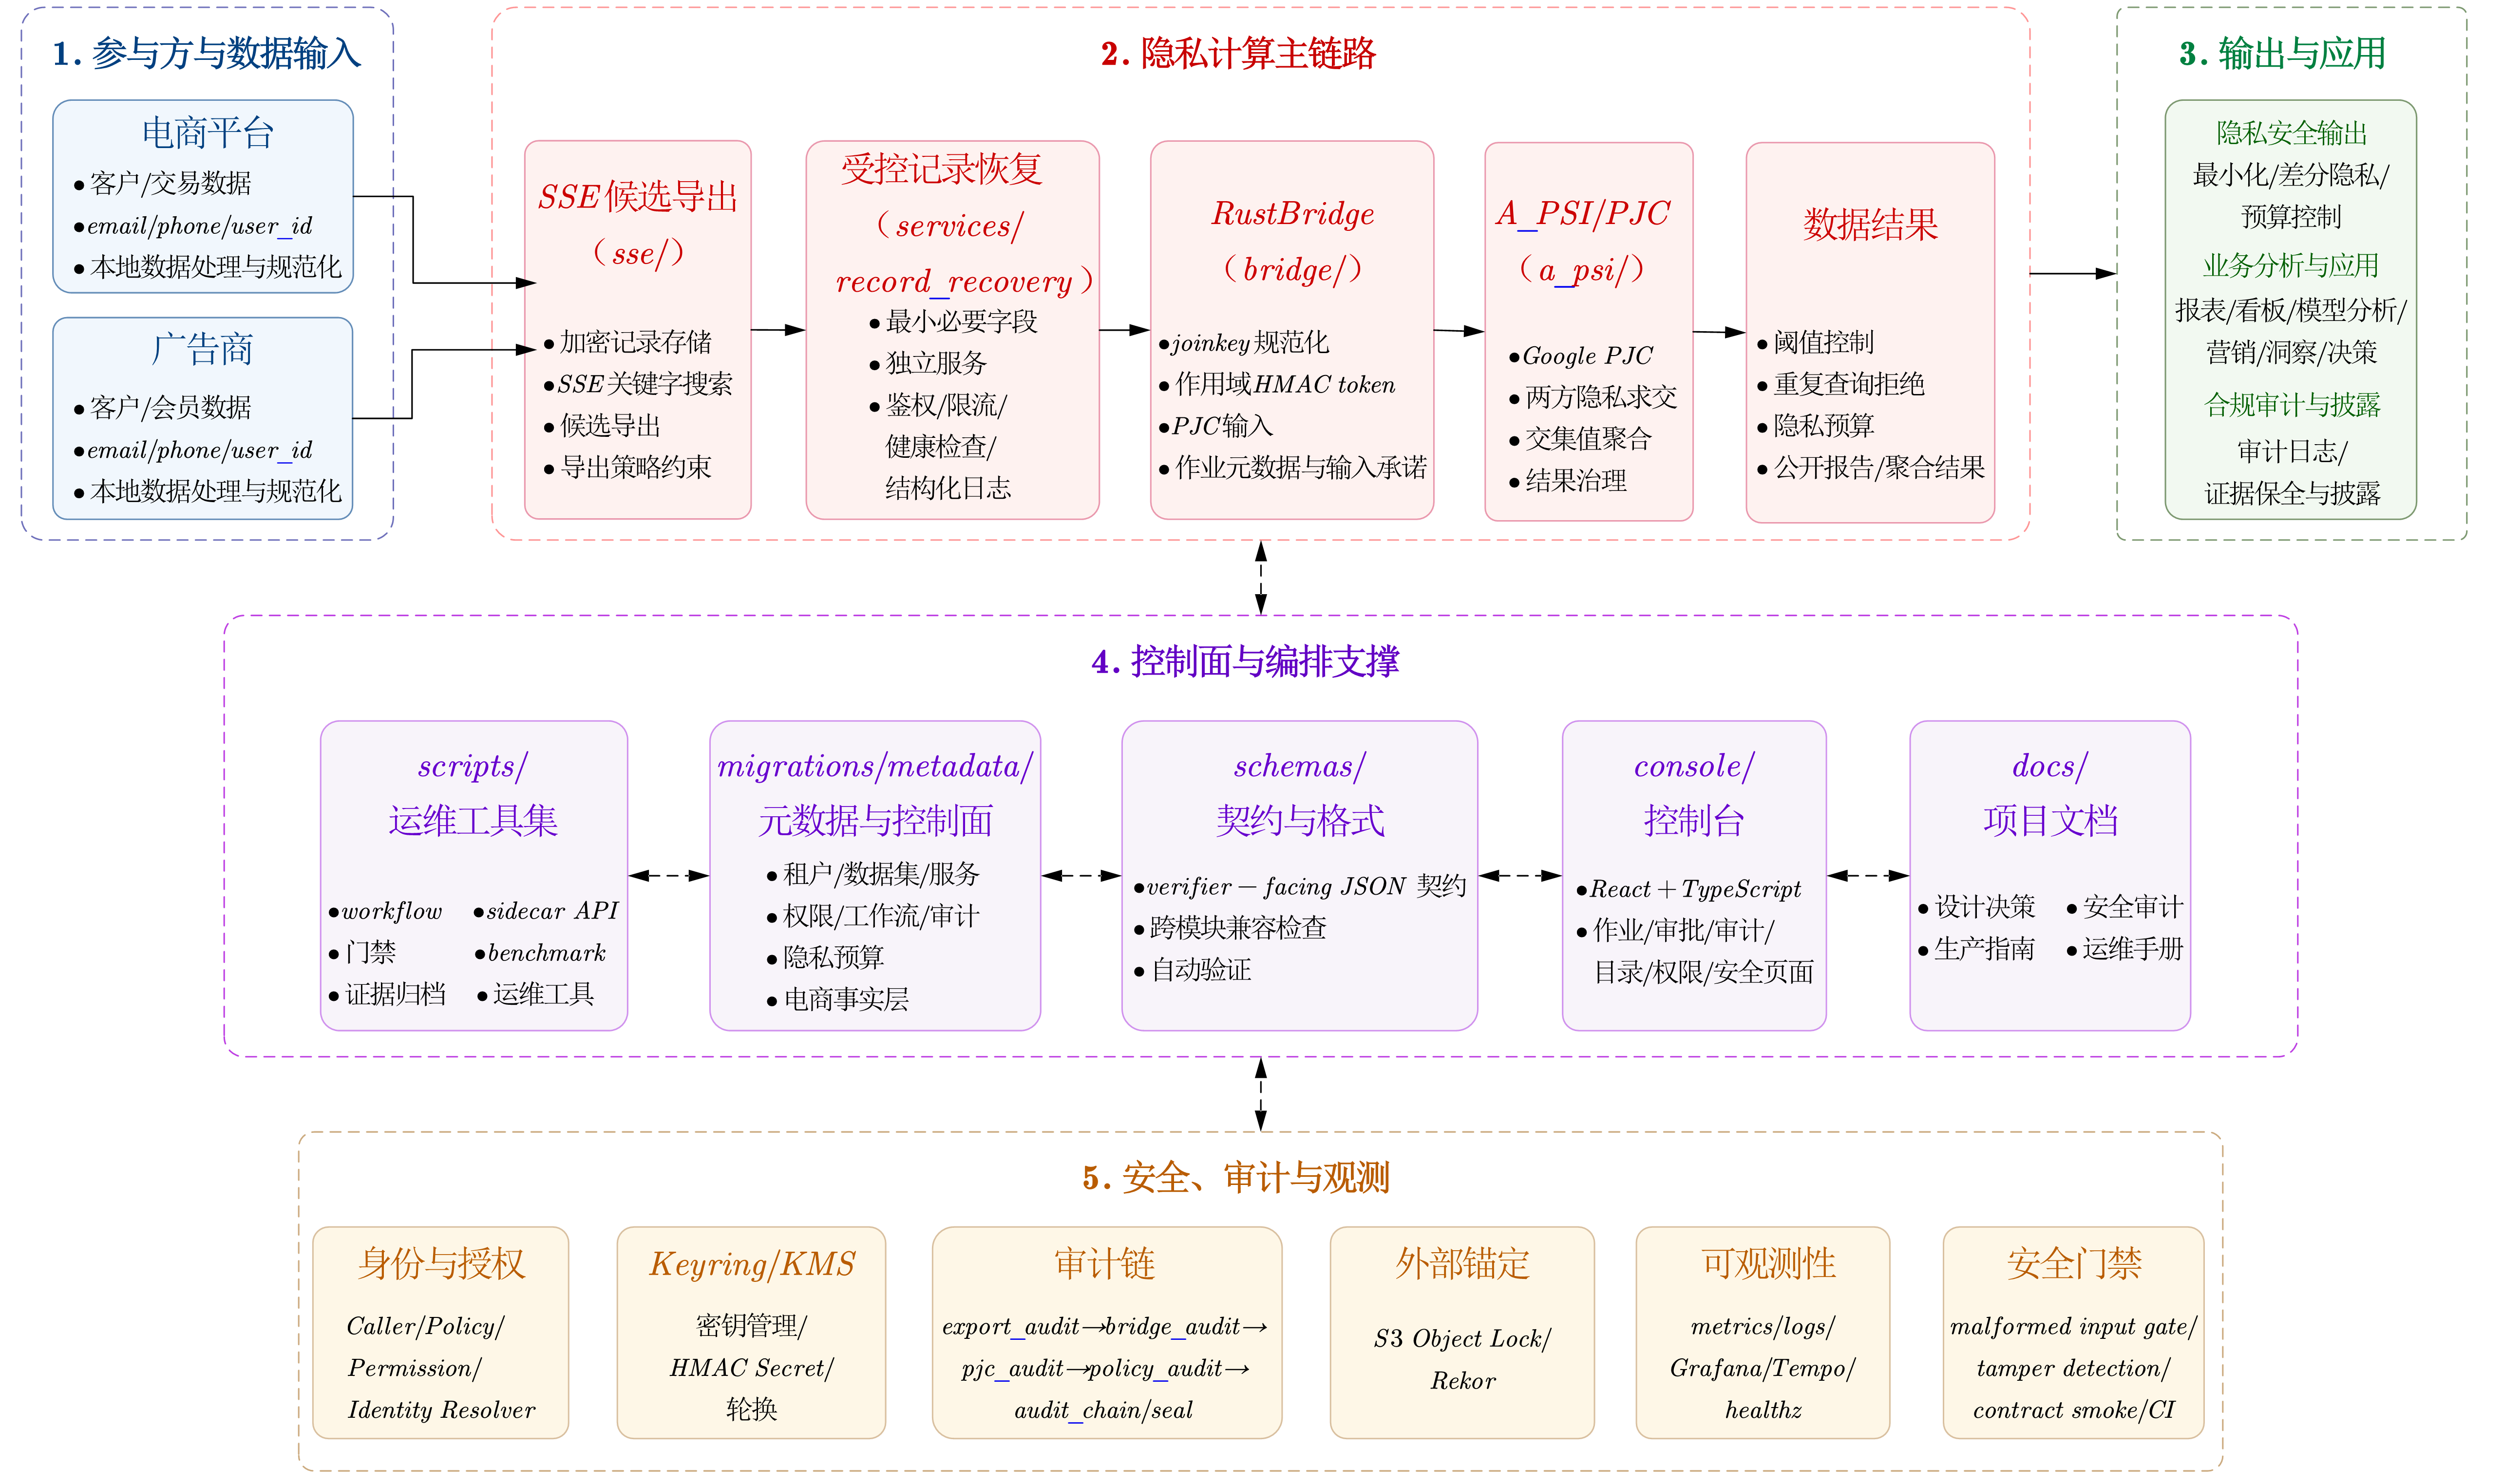
\includegraphics[width=\textwidth]{信安赛.png}
    \caption{面向电商隐私分析场景的 SSE 与 PJC 平台总体架构}
    \label{fig:platform-architecture}
\end{figure}

\chapter{关键模块设计与实现}

\section{SSE 模块}

\subsection{设计目标}

SSE 模块用于在不直接暴露数据库明文内容的情况下，根据关键字返回候选记录标识。它承担主链路中的 candidate selection，而不是直接完成最终跨方计算。通过先筛选候选集合，系统能够减少后续恢复与 PJC 的处理范围。

\subsection{核心机制}

系统将敏感记录写入加密记录库，并为可检索字段建立 SSE 索引。调用方提交查询后，SSE 服务返回候选标识，再由 export policy 校验 caller、role、join key、value field、过滤字段和最大行数。候选导出结果附带任务、作用域和哈希信息，为恢复和 Bridge 阶段提供约束。

旧版 SSE WebSocket 网络暴露面已经退休，其中网络 pickle 类远程代码执行风险已被移除并由门禁覆盖。保留的核心能力是加密索引和候选筛选。

\subsection{当前边界}

SSE 会泄露一定的搜索模式、访问模式与候选数量。当前实现没有使用 ORAM、forward-private SSE 或 OPRF-blinded query，因此不能声称解决了所有检索泄露问题。项目通过访问控制、查询治理和审计降低滥用风险，但更强泄露模型仍需替换或增强底层协议。

\section{Record Recovery 模块}

\subsection{设计目标}

候选标识本身不能直接用于 PJC。Record Recovery 模块在策略允许的范围内，从加密记录库恢复 join key 和必要 value 字段，并阻止任意记录扫描和非必要字段扩散。

\subsection{实现机制}

加密记录库使用 PBKDF2HMAC-SHA256 派生密钥、AES-256-GCM 加密记录，并使用 keyed HMAC-SHA256 生成记录标识标签。恢复逻辑位于独立的 \filepath{services/record_recovery/} 服务边界，支持 subprocess、Unix socket 和 HTTP transport。HTTP 模式包含请求签名、时间戳防重放、caller 级限流、最大请求行数、mTLS 配置、健康检查和 Prometheus 指标。

恢复请求必须绑定 caller、tenant、dataset、service 和 job；生产门禁还要求显式配置 output root、record-store root 和最大行数，避免使用不受控默认路径。

\subsection{安全意义}

独立恢复服务将 ``能够搜索候选'' 与 ``能够读取敏感字段'' 分离。即使查询端获得候选标识，也必须经过恢复服务的授权和审计才能取得最小必要数据。该设计缩小了明文出现范围，并使恢复行为能够单独限流、监控和取证。

\section{Bridge 模块}

\subsection{设计目标}

Bridge 位于原始标识与 PJC 输入之间，目标是消除格式差异、避免直接传递 join key，并确保后续计算输入与任务上下文一致。

\subsection{实现机制}

Bridge 使用 Rust 实现，对 email、phone 和普通 id 执行确定性规范化，再使用作用域约束的 HMAC-SHA256 生成 token。作用域包含任务和数据域信息，使同一原始标识在不同作用域中不能被简单关联。Bridge 生成 server/client CSV、job metadata、审计事件和 input commitment。

输入承诺覆盖 Bridge 输出和关键元数据。PJC 执行及 release gate 会检查承诺绑定，从而发现 Bridge 之后的 CSV 或 manifest 被替换、篡改的情况。Bridge token secret 不应出现在命令行、日志或审计产物中，生产模式通过 key agent 或外部 KMS adapter 获取密钥。

\subsection{安全意义}

Bridge 将跨方计算对象从可识别的原始 join key 转换为任务作用域 token，并通过输入承诺连接数据准备、PJC 计算和结果发布。它降低了标识泄露与跨任务关联风险，也提高了中间产物可验证性。

\section{Google PJC 模块}

\subsection{设计目标}

PJC 模块负责在双方不直接交换集合成员的情况下，计算 token 集合交集大小以及交集上 client value 的聚合值。典型场景是广告侧作为 server 提供曝光集合，电商侧作为 client 提供转化用户与金额。

\subsection{实现机制}

系统集成 Google Private Join and Compute 实现，提供 server/client 双方运行脚本、TLS 与 mTLS 配置、分桶与分片流程、结果合并、输入承诺检查和发布前验证。为突破百万级输入下单一 gRPC 消息大小限制，项目增加了兼容的流式 gRPC 路径，并支持按块传输重复加密集合。

\subsection{边界说明}

当前 PJC 安全边界必须表述为 \textbf{semi-honest/operator-controlled}。系统能够发现 repo-side 路径中的输入篡改，并能通过来源证明和双人签署增强协议外治理，但不能阻止恶意参与方偏离协议、伪造源数据或提交任意数值。若要声称 malicious-secure，需要采用恶意安全 PSI-SUM、2PC/MPC 后端或引入有效的范围证明和值证明。

\section{Control Plane 与 Query Workflow}

\subsection{Metadata Sidecar}

Metadata Sidecar 使用 SQLite/PostgreSQL 双后端记录租户、数据集、服务、调用方、角色、策略、密钥注册、作业、阶段状态、审计事件和隐私预算。它不默认保存完整订单明细，而是作为控制面回答 ``谁在什么作用域下运行了什么任务、经过了哪些决策、产生了哪些证据''。

\subsection{Query Workflow}

Query Workflow 将请求提交、审核、批准、入队、worker 执行、结果发布和状态回写连接为闭环。审批流程禁止同一身份自批，审批与隐私预算消费会写入控制面变更记录。默认发布路径对预算并发扣减和一次性近似查询审批消费采用事务化存储，避免重复消费和并发双花。

\subsection{Operator Surface}

Operator Console 是基于 Vite、React 和 TypeScript 的单页应用，覆盖 home、jobs、requests、audit、catalog、permissions、recovery、observability、compliance、security 和 settings 等操作面。控制台能够发起完整主链路任务、独立 SSE 查询和独立 PJC 任务，并展示公开摘要、审计证据和平台健康状态。

\chapter{安全设计与治理机制}

\section{安全目标}

项目重点保护原始 join key、业务明细、token secret、记录库密钥和未发布的计算结果；限制越权恢复、过细结果、重复查询和中间产物替换；并为每个关键决策提供可验证证据。系统不承诺隐藏所有 SSE 访问模式，也不承诺在恶意协议参与者或被完全控制的外部信任根下仍然安全。

\section{威胁模型}

系统考虑以下威胁：

\begin{enumerate}
  \item \textbf{查询滥用：}调用方通过重复、近似或过细查询推断个体信息。
  \item \textbf{越权恢复：}服务调用方绕过候选范围或恢复不必要字段。
  \item \textbf{中间产物篡改：}Bridge 输出、作业清单、PJC 结果或审计文件被替换。
  \item \textbf{网络与接口攻击：}恶意输入、重放、错误签名、TLS 配置错误和资源耗尽。
  \item \textbf{恶意参与者：}PJC 一方伪造源数据、偏离协议或提交异常 value。
  \item \textbf{运维侧风险：}管理员、身份系统、KMS 或审计锚点被滥用或配置错误。
\end{enumerate}

\section{协议内与协议外边界}

协议内安全关注 SSE、令牌化和 PJC 本身能够隐藏什么，以及参与方需要遵守哪些假设。协议外治理关注谁批准任务、源数据是否有责任人签署、发布是否满足预算、证据是否归档和外部信任根是否真实可用。

本项目的 source export manifest、source attestation、双人签署、input commitment、release governance report 和 external anchor 属于协议外治理。它们能够减少未授权发布和无证据运行，但不会把半诚实 PJC 自动提升为恶意安全协议。

\section{当前已实现的安全增强}

\begingroup
\renewcommand{\arraystretch}{1.3}
\begin{longtable}{%
  >{\raggedright\arraybackslash}p{0.26\textwidth}%
  @{\hspace{0.02\textwidth}}%
  >{\raggedright\arraybackslash}p{0.64\textwidth}%
}
\caption{当前已实现的安全增强机制}\label{tab:security-controls}\\
\toprule
\textbf{机制} & \textbf{作用} \\
\midrule
\endfirsthead
\caption[]{当前已实现的安全增强机制（续）}\\
\toprule
\textbf{机制} & \textbf{作用} \\
\midrule
\endhead
\bottomrule
\endfoot
\bottomrule
\endlastfoot
Input Commitment & 绑定 Bridge 输出、作业元数据、PJC 执行与发布结果，检测 repo-side 输入替换。 \\
Source Attestation & 绑定源导出清单、作用域、双人签署与 reviewer separation，证明发布所依据的数据来源。 \\
Release Gate & 检查阈值、签署、来源真实性、输入承诺、外部锚点和发布策略。 \\
Privacy Budget & 限制重复、近似、时间窗口相近、阈值取整和跨 bucket 差分查询。 \\
Audit Chain 与 Seal & 串联阶段事件并生成密封证据，支持 bit-flip 篡改检测、归档与恢复验证。 \\
External Anchor & 支持本地 ledger、S3 Object Lock 和 Sigstore Rekor 透明日志适配。 \\
Identity 与 Authorization & 支持 caller scope、OIDC/JWKS、OpenFGA 风格关系和业务访问策略。 \\
Negative Security Gates & 覆盖恶意 HTTP 输入、重放、错误签名、网络 pickle、审计篡改和资源 fail-closed。 \\
\end{longtable}
\endgroup

\section{当前仍然保留的边界}

首先，PJC 仍基于半诚实参与方假设，无法证明参与方提交的源数据和值真实，也无法阻止协议主动偏离。其次，SSE 的访问模式和搜索模式泄露尚未通过更强协议解决。再次，真实 Keycloak、OpenFGA、Vault、云 KMS、不可变审计锚点和高可用 PostgreSQL 的长期托管、轮换、吊销与 SRE 流程属于外部企业信任根，仓库只能提供 adapter、门禁和证据收集工具，不能代替真实生产运维。

\chapter{电商叙事环境与业务适配}

\section{为什么选择电商场景}

电商数据天然分布在多个主体和业务域中。广告平台拥有曝光与点击，商家拥有订单与商品，支付方拥有交易状态，物流方拥有履约节点，客服系统拥有售后记录。跨方分析价值高，但用户标识、金额和行为链路敏感，适合展示隐私计算对 ``可用不可见'' 的支持。

本项目可支持广告归因、复购分析、风险名单交集、客服回访范围筛选和合规审计等场景。输出通常是交集数量、成交金额或受阈值保护的聚合，而非交集成员清单。

\section{电商事实层适配}

控制面迁移中提供 orders、order items、order attribution、order payment、order fulfillment 和 customer service interactions 六类事实表基线，并增加 buyer、merchant staff、customer service agent、courier 和 field marketer 等业务身份注解。业务访问策略能够描述 persona、资源、目的和字段级访问约束，控制台提供 business-access workbench 和公开摘要检查。

这些事实表和身份模型用于证明平台能够承载真实业务语义，但不意味着项目已成为完整交易系统。敏感业务事实仍应由实际业务系统负责，隐私平台只获取经过授权的必要输入。

\section{电商叙事与技术主线的关系}

电商是平台的重要业务适配场景，数据库/控制面 + SSE + Google PJC 才是技术主线。将两者区分能够避免把事实表数量或控制台页面数量误当作隐私协议安全性。项目价值在于：使用电商场景说明隐私计算主链路如何进入真实业务流程，并通过控制面、审批和证据治理降低落地风险。

\chapter{系统验证与实验结果}

\section{验证方法}

项目采用分层验证方法：

\begin{enumerate}
  \item 使用 \filepath{schemas/} 中的 JSON Schema 固化模块输入、输出和 verifier evidence。
  \item 通过 contract smoke 与 schema back-compat 检查接口完整性和兼容性。
  \item 通过端到端 demo 验证 SSE、recovery、Bridge、PJC 和 release 主链路。
  \item 通过 malformed input、audit tamper、anti-replay、权限拒绝和 chaos drill 验证失败路径。
  \item 通过 SSE export、record recovery、Bridge、PJC、完整管线和数据库 adapter benchmark 验证性能。
  \item 通过 deployment evidence gate、live archive 和 production security closure gate 汇总 repo-side 与 live-side 状态。
\end{enumerate}

\section{关键结果}

\begingroup
\renewcommand{\arraystretch}{1.3}
\begin{longtable}{%
  >{\raggedright\arraybackslash}p{0.30\textwidth}%
  @{\hspace{0.02\textwidth}}%
  >{\raggedright\arraybackslash}p{0.58\textwidth}%
}
\caption{系统关键验证与实验结果}\label{tab:key-results}\\
\toprule
\textbf{验证项} & \textbf{结果} \\
\midrule
\endfirsthead
\caption[]{系统关键验证与实验结果（续）}\\
\toprule
\textbf{验证项} & \textbf{结果} \\
\midrule
\endhead
\bottomrule
\endfoot
\bottomrule
\endlastfoot
标准端到端示例 & \texttt{intersection\_size=2}，\texttt{intersection\_sum=425}。 \\
顶层闭环状态 & 16 个 verifier-facing 模块全部达到 \texttt{repo\_side\_status=ok} 与 \texttt{live\_status=ok}，live fail 为 0。 \\
SSE Export 规模 & 已完成 100k 与 1M candidates 本地规模测试。 \\
Record Recovery & 1k candidates、10 路 HTTP 并发测试吞吐为 15.818 req/s。 \\
Rust Bridge & 100k/100k 输入约 0.366 秒；1M/1M 输入约 4.437 秒。 \\
PJC 规模 & 100k/100k 测试约 222.02 秒；流式 1M/1M 测试约 34 分 05 秒，峰值 RSS 约 2.20 GB，并成功输出结果。 \\
主链路 SLO & 10k 规模完整管线约 34.9 秒，结果与预期一致。 \\
安全负向测试 & malformed HTTP 输入、审计 bit-flip 篡改、错误签名、重放和网络 pickle 风险均有自动门禁。 \\
\end{longtable}
\endgroup

标准主链路可以通过以下命令运行：

\begin{lstlisting}[language=bash]
bash scripts/run_live_sse_bridge_demo.sh
bash scripts/check_json_contracts.sh
bash scripts/check_ci_smoke.sh
\end{lstlisting}
  \section{CPU 核数与内存容量对性能的影响分析}

  为评估系统在不同部署资源条件下的运行表现，本文对 SSE Export 与 PJC 两个关键模块进行了 CPU--Memory 资源矩阵 benchmark。
  实验重点关注两个方面：一是 CPU 核数和内存容量变化对模块吞吐量的影响；二是在资源不足时，系统是否会出现明显的失败边界。
  该实验用于辅助判断系统部署时的资源需求、扩展收益和资源隔离策略。

  \subsection{SSE Export 性能分析}

  SSE Export 测试采用 20,000 条 candidates 作为输入规模，在 1、2、3、4、5、6、8、12、16 核和 64 MB 至 768 MB 内存限制下
  进行测试。每个资源点重复运行 3 次，共完成 243 次真实测量，全部运行成功。

  实验结果显示，SSE Export 的峰值 RSS 稳定在约 43 MB，说明该规模下 64 MB 内存限制已经能够容纳工作集。不同内存上限下的吞
  吐量差异较小，整体 p50 吞吐量主要分布在 20,000 records/s 左右，未观察到随内存增加而持续提升的趋势。

  从 CPU 核数角度看，SSE Export 在 1 核至 16 核之间也没有形成稳定的线性加速。各 CPU 档位的 p50 吞吐量中位数大致位于
  20.1k--20.6k records/s 区间。该现象说明当前 SSE Export 路径主要受单进程记录处理、加密记录读取和输出写入影响，增加 CPU
  核数不能显著提升吞吐。

  因此，SSE Export 的部署重点不是盲目增加 CPU 或内存，而是保证基础内存能够覆盖加密记录与候选集合工作集，并优化单进程处理
  路径、I/O 路径和批量导出流程。

  \begin{figure}[H]
  \centering
  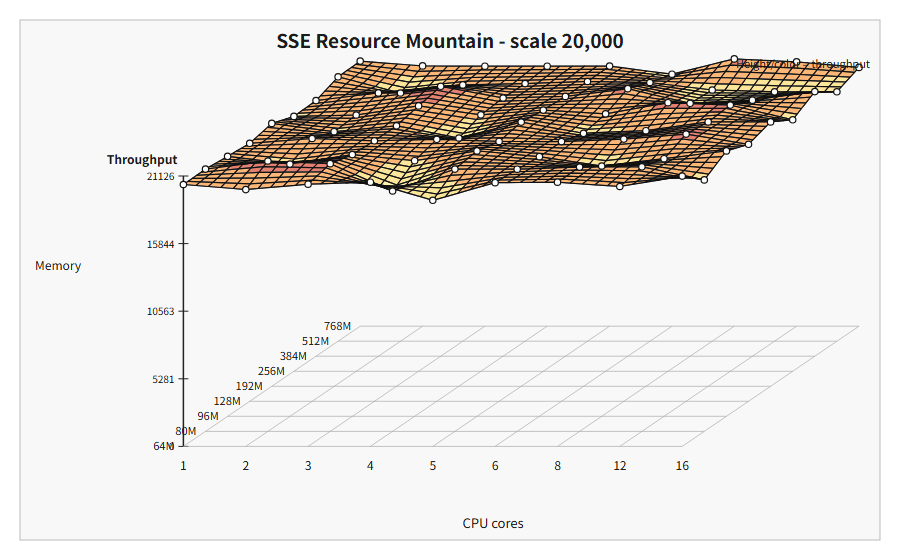
\includegraphics[width=0.92\textwidth]{sse_resource_mountain.png}
  \caption{SSE Export 在不同 CPU 核数与内存上限下的三维性能曲面}
  \label{fig:sse-resource-mountain}
  \end{figure}

  \begin{figure}[H]
  \centering
  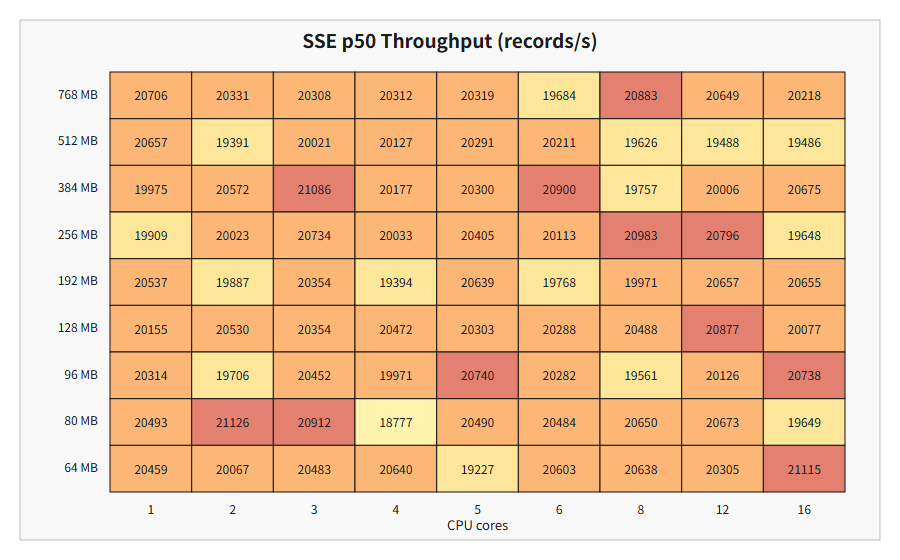
\includegraphics[width=0.92\textwidth]{sse_resource_heatmap.png}
  \caption{SSE Export 在不同 CPU 核数与内存上限下的吞吐量热力图}
  \label{fig:sse-resource-heatmap}
  \end{figure}

  \subsection{PJC 性能分析}

  PJC 测试采用 1,000 $\times$ 1,000 的双方输入规模，对 1、2、4、6、8、16 核以及 512 MB、768 MB、1024 MB、1536 MB、2048
  MB、4096 MB 内存限制进行测试。基础矩阵共包含 36 个资源点，其中 15 个资源点成功，21 个资源点失败。失败点主要集中在低内
  存区域。

  从内存容量角度看，PJC 对地址空间限制更加敏感。在 2 核条件下，512 MB、768 MB 和 1024 MB 三个内存档均为 0/3 成功；而
  1536 MB、2048 MB 和 4096 MB 均为 3/3 成功。该结果表明，在当前端到端 PJC runner 中，稳定运行所需的地址空间下限约为 1.5
  GB。

  需要注意的是，PJC 成功运行时的峰值 RSS 约为 15--16 MB，但 1 GB 地址空间限制下仍稳定失败。这说明仅观察 RSS 容易低估 PJC
  的资源需求；部署时应同时关注虚拟地址空间限制、超时成功率和端到端完成时间。

  从 CPU 核数角度看，PJC 并未表现出随核心数量增加而稳定提升的趋势。在 1536 MB 内存限制下，1、2、4、8、16 核的成功率分别
  为 2/3、3/3、3/3、2/3、3/3，对应 p50 吞吐量约为 45.6、90.8、36.0、53.8、75.0 items/s。其中 2 核表现最好，继续增加核心
  没有带来稳定收益。

  这一结果与当前 PJC 运行方式有关。系统以本地 server/client 两个进程执行 PJC，并通过回环 gRPC 通信。端到端运行还包含密码
  学密钥生成、进程启动和网络通信开销。部分失败日志停留在 \texttt{Client: Generating keys...} 阶段，说明密钥生成的随机长
  尾会显著影响端到端耗时。因此，本实验反映的是 PJC 端到端部署路径的性能，而不是单独协议计算阶段的理论并行加速能力。

  \begin{figure}[H]
  \centering
  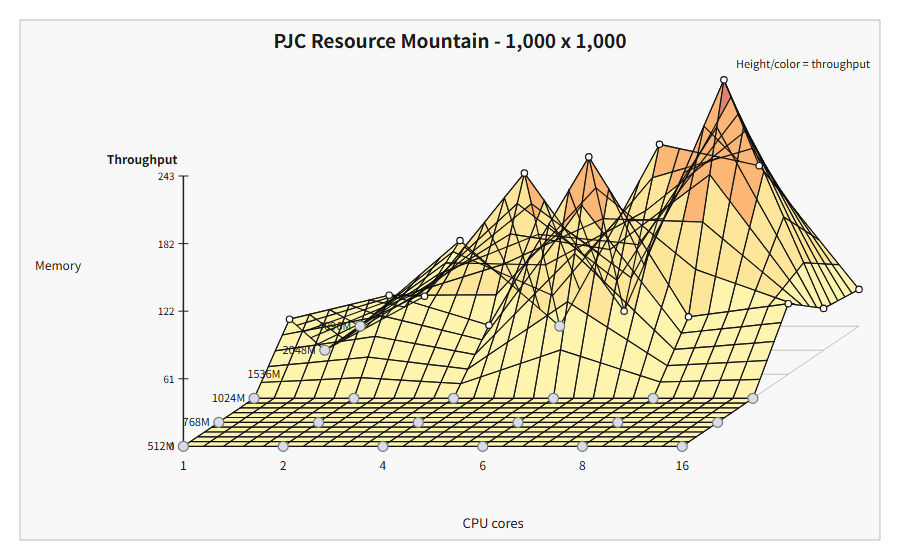
\includegraphics[width=0.92\textwidth]{pjc_resource_mountain.png}
  \caption{PJC 在不同 CPU 核数与内存上限下的三维性能曲面}
  \label{fig:pjc-resource-mountain}
  \end{figure}

  \begin{figure}[H]
  \centering
  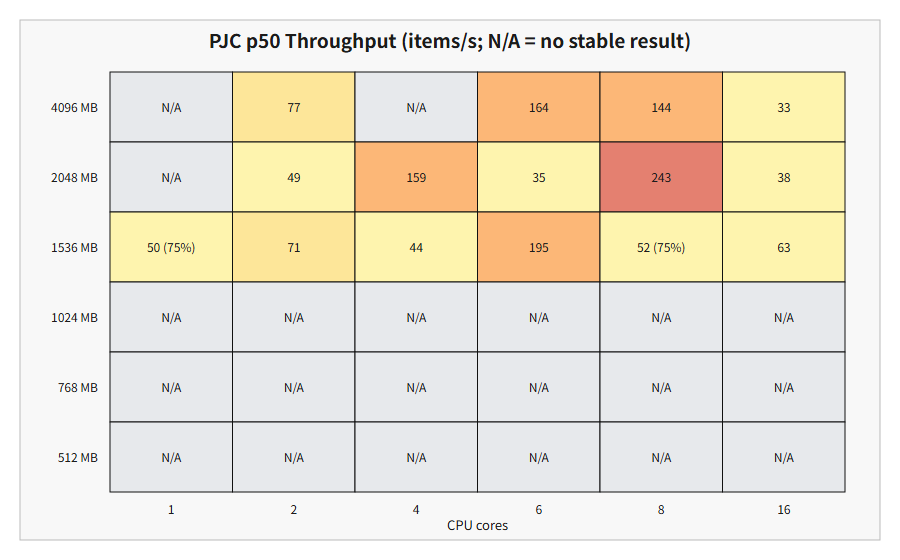
\includegraphics[width=0.92\textwidth]{pjc_resource_heatmap.png}
  \caption{PJC 在不同 CPU 核数与内存上限下的吞吐量与失败区域热力图}
  \label{fig:pjc-resource-heatmap}
  \end{figure}

  \subsection{SSE 与 PJC 对比分析}

  SSE Export 与 PJC 在资源敏感性上表现出明显差异。SSE Export 的工作集较小，在 64 MB 内存限制下即可稳定运行，且增加 CPU
  核数和内存容量带来的收益有限。PJC 则对地址空间更加敏感，在 1 GB 以下出现明显失败区间，约 1.5 GB 后才进入稳定可运行区
  域。

  从吞吐稳定性看，SSE Export 的性能曲面较为平坦，说明其瓶颈主要来自串行处理和 I/O 路径；PJC 的性能曲面更不平滑，既受到地
  址空间限制影响，也受到密钥生成、server/client 调度和 gRPC 通信开销影响。

  综合来看，系统部署时应采用差异化资源策略。SSE 模块可优先关注 I/O、批处理和单进程优化；PJC 模块则应预留更充足的地址空
  间，并通过超时控制、任务重试、分桶分片和进程隔离提高端到端成功率。

  \subsection{性能分析结论}

  资源矩阵 benchmark 表明，SSE Export 在当前规模下具备稳定的资源表现，低内存条件下也能完成候选导出；PJC 是更需要重点规划
  资源的模块，其稳定运行依赖更高的地址空间上限，并且端到端性能受密钥生成和双进程通信路径影响较大。

  因此，在实际部署中，SSE 可作为轻量候选筛选与导出模块进行横向任务调度，而 PJC 应作为资源敏感型计算模块单独配置资源限
  额、超时策略和失败重试机制。该结果为后续平台容量规划、SLO 设定和生产部署参数选择提供了依据。
\section{模块级状态汇总}

\begingroup
\renewcommand{\arraystretch}{1.3}
\begin{longtable}{%
  >{\raggedright\arraybackslash}p{0.23\textwidth}%
  @{\hspace{0.015\textwidth}}%
  >{\raggedright\arraybackslash}p{0.18\textwidth}%
  @{\hspace{0.015\textwidth}}%
  >{\raggedright\arraybackslash}p{0.48\textwidth}%
}
\caption{模块级完成状态汇总}\label{tab:module-status}\\
\toprule
\textbf{模块类别} & \textbf{状态} & \textbf{说明} \\
\midrule
\endfirsthead
\caption[]{模块级完成状态汇总（续）}\\
\toprule
\textbf{模块类别} & \textbf{状态} & \textbf{说明} \\
\midrule
\endhead
\bottomrule
\endfoot
\bottomrule
\endlastfoot
核心主链路 & 已完成 & SSE、recovery、Bridge、PJC、release 可端到端运行并验证。 \\
控制面与工作流 & 已完成 & Metadata、请求审批、worker、隐私预算和 operator console 已形成闭环。 \\
契约与审计 & 已完成 & Typed schema、审计链、seal、archive、public summary 和 external anchor adapter 可用。 \\
部署与 live evidence & 已收口 & 顶层 16 个 verifier-facing 模块 live status 均为 ok。 \\
协议安全等级 & 保留边界 & PJC 仍为 semi-honest/operator-controlled，不声称 malicious-secure。 \\
企业长期运维 & 外部依赖 & 真实身份根、KMS、HA、不可变锚点和 SRE 托管需在目标环境持续运行。 \\
\end{longtable}
\endgroup

\section{客观评价}

从工程完成度看，项目已超过单一算法 demo，形成了协议、服务、控制面、前端、验证和运维证据组成的平台工程。从平台化程度看，typed schema、workflow、sidecar、公开摘要和 live evidence gate 使系统具备较强的可解释性与可复现性。从协议安全角度看，输入承诺和协议外治理显著降低了 repo-side 篡改与无审批发布风险，但没有改变 PJC 的半诚实假设。从答辩和展示价值看，项目能够以清晰的电商场景呈现隐私计算从候选筛选到结果发布的完整过程，并能够客观说明能力边界。

\chapter{不足与改进方向}

\section{当前不足}

\begin{enumerate}
  \item PJC 不能抵抗恶意参与方主动偏离协议、伪造集合或提交异常 value。
  \item SSE 仍可能泄露搜索模式、访问模式和候选规模。
  \item 百万级 PJC 虽已通过流式传输完成，但耗时与内存占用仍较高，继续扩展需要分片、资源隔离和协议优化。
  \item 真实企业身份根、密钥管理、不可变审计锚点、数据库高可用和长期 SRE 不是代码仓库自身能够完全解决的问题。
  \item 电商事实层和身份模型是适配基线，不覆盖完整业务域和组织权限体系。
\end{enumerate}

\section{不更换协议前提下的改进方向}

在保持现有协议主线的前提下，可继续加强 source attestation 的外部签署与轮换机制，扩大 release gate 对近似查询和跨任务差分的识别能力，使用真实 PostgreSQL 与队列提升 workflow 持久性，完善 PJC 资源限额与 fail-closed 策略，并在目标环境持续收集 mTLS、KMS、HA、外部锚点和灾备演练证据。

性能方面，可进一步进行 PJC 分桶并行、内存热点分析、重复连接复用和多租户资源调度；运维方面，可将控制台、告警、审计归档和证据刷新纳入标准化发布流水线。

\section{必须超出当前框架才能解决的问题}

若要抵抗恶意计算参与方，需要引入 malicious-secure PSI-SUM、主动安全 MPC/2PC、零知识范围证明或可信执行环境等新能力。若要显著降低 SSE 搜索与访问模式泄露，需要采用 ORAM、forward-private SSE、OPRF 盲化查询等更强方案。若要形成真正的生产信任根，则必须由外部组织长期运营身份系统、KMS、不可变存储、审计机构和高可用基础设施。

\chapter{结论}

本文围绕跨方电商隐私分析问题，设计并实现了一个由数据库/控制面、SSE、受控记录恢复、Rust Bridge、Google PJC 和策略发布构成的隐私计算平台。系统不仅能够完成候选筛选、集合求交和聚合计算，还通过作用域授权、输入承诺、来源证明、隐私预算、审批流、审计链、外部锚点和 verifier evidence 建立了协议外治理闭环。

项目验证表明，标准主链路能够稳定得到预期结果，模块契约、失败路径、规模性能和 live evidence 均具备自动化验证入口。平台级收口已经完成，但核心计算仍遵循半诚实参与方与受控运维环境假设。该项目的主要意义在于将隐私计算算法转化为可运行、可治理、可审计的平台工程，并以清晰、客观的方式说明其能力与边界，为后续接入恶意安全协议和真实企业信任根提供了基础。

\appendix

\chapter{主要验证命令}

\begin{lstlisting}[language=bash]
# 端到端主链路
bash scripts/run_live_sse_bridge_demo.sh

# JSON 契约与 CI smoke
bash scripts/check_json_contracts.sh
bash scripts/check_ci_smoke.sh
python3 scripts/check_schema_backcompat.py

# 安全负向测试
python3 scripts/check_http_malformed_input_gate.py
python3 scripts/verify_audit_tamper_resistance.py --help

# Benchmark 入口
python3 scripts/benchmark_smoke.py --help
python3 scripts/benchmark_pjc.py --help
\end{lstlisting}

\chapter{关键证据与文档入口}

\begingroup
\renewcommand{\arraystretch}{1.3}
\begin{longtable}{%
  >{\raggedright\arraybackslash}p{0.36\textwidth}%
  @{\hspace{0.02\textwidth}}%
  >{\raggedright\arraybackslash}p{0.54\textwidth}%
}
\caption{关键证据与文档入口}\label{tab:evidence-documents}\\
\toprule
\textbf{路径} & \textbf{用途} \\
\midrule
\endfirsthead
\caption[]{关键证据与文档入口（续）}\\
\toprule
\textbf{路径} & \textbf{用途} \\
\midrule
\endhead
\bottomrule
\endfoot
\bottomrule
\endlastfoot
\filepath{README.md} & 项目定位、功能、安装与主链路运行说明。 \\
\filepath{docs/COMPACT_PLATFORM_BRIEF.md} & 平台能力、当前状态和关键边界压缩总览。 \\
\filepath{docs/CURRENT_SECURITY_AND_COMPLETION_AUDIT.md} & 当前权威安全与完成度判断。 \\
\filepath{docs/PRODUCTION_READINESS_GUIDEBOOK.md} & 部署、性能、运维和生产就绪验证记录。 \\
\filepath{docs/THREAT_MODEL_AND_LEAKAGE_MODEL.md} & 威胁模型和阶段泄露边界。 \\
\filepath{schemas/} & 所有 verifier-facing typed contract。 \\
\filepath{scripts/} & 主链路、门禁、benchmark 与证据归档入口。 \\
\end{longtable}
\endgroup

\end{document}
